\titre{Ressource :} 
	\begin{itemize}
		\item wiki-du-lama
		\item Systèmes d'exploitation (A. Tanenbaum) chap 2 et 6
	\end{itemize}

\titre{Définition :} La multiprogrammation, c'est exécuter simultanément plusieurs programmes sur une même machine, un même CPU, en basculant rapidement de l'un à l'autre, créant une impression de simultanéité. \\

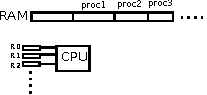
\includegraphics[width=200px]{fig1.pdf}

\begin{tabular}{cccc}
	 & Proc1 & Proc2 & Proc3 \\ \hline
	R0 & $\ldots$ & $\ldots$ & $\ldots$ \\
	R1 & $\ldots$ & $\ldots$ & $\ldots$\\
	$\ldots$ & $\ldots$ & $\ldots$ & $\ldots$
\end{tabular}

\titre{Processus :} Un programme en cours d'exécution

\titre{2 composantes principales :}
\begin{itemize}
	\item Espace d'adressage (mémoire) : code, données, pile
	\item Registres : valeurs
\end{itemize}

\titre{Préemption :} Action d'interrompre l'exécution d'un processus avec l'intention de la reprendre plus tard. \\
\titre{Rq :} La coopération du processus n'est pas requise, et le processus ne "sait" pas qu'il est préempté. \\

\titre{Rq :} On ne connait pas l'ordonnanceur. On ne peut faire aucune supposition sur ce qu'il fera. \\

\titre{Causes de la préemption :}
\begin{enumerate}
	\item A la demande du processus (sleep, $\ldots$)
	\item Appel système (ex : utilisation d'un périphérique)
	\item Déclenchement d'une interruption (par l'horloge, par un périphérique etc.)
\end{enumerate}

\titre{Exemple wiki} \\

\titre{Exemple : x = x + 1} voir figure 2 incomplète\\

\titre{Conclusion :} 
\begin{enumerate}
	\item Prudence lorsque deux processus simultanés manipulent les même données
	\item Difficulté de debuggage car les erreurs dépendent de l'ordonnanceur, qu'on ne maîtrise pas.
\end{enumerate}

\titre{Condition de concurrence :} C'est une situation où deux processus (ou plus) manipulent des données partagées et où le résultat final dépend de l'ordre d'exécution.

\titre{Exemple :} Spool d'impression : \\
Un tableau contenant les documents et un compteur prochainLibre. \\
3 étapes pour imprimer : 
\begin{itemize}
	\item Lire ProchainLibre
	\item Ecrire le doc dans cette case
	\item Incrémenter prochainLibre
\end{itemize}
PL = 10 \\

\underline{ProcA :}\\
Lit 10\\
Ecrit le doc dans 10\\
\underline{ProcB :}\\
Lit 10\\
Ecrit le doc dans 10\\
\underline{ProcA :}\\
PL = 11\\
\underline{ProcB :}\\
PL = 11\\

\titre{Section critique :} Partie du code dans laquelle deux processus ne doivent jamais se trouver simultanément. \\

\newpage

\titre{Deux objectifs :} 
\begin{enumerate}
	\item Identifier les sections critiques
	\item S'assurer qu'il n'y a jamais deux processus sur ces sections ( Assurer l'exclusion mutuelle )
\end{enumerate} 

\titre{Problème :}
Si un code source manipules des variables locales dans cet ordre : Comment sont les sections critiques ?
$$
\begin{array}{ccccc}
L-&P-&L-&P-&L- \ldots \\
 -&C-& -&C-& - \ldots ? \\
 -&  &C & -& - \ldots ?
\end{array}
$$ 

\titre{Les 4 règles d'or}
\begin{enumerate}
	\item Deux processus ne doivent jamais se trouver simultanément en section critique
	\item Il ne faut jamais faire de supposition quand à la vitesse et au nombre de processus en oeuvre
	\item Aucun processus s'exécutant en section critique ne doit bloquer les autres (ie : il faut se dépêcher de quitter la section critique)
	\item Aucun processus ne doit attendre indéfiniment l'accès à une section critique.
\end{enumerate}


